\section{Rotação de um Objeto Sobre um Eixo Fixo}
\subsection{Conteúdo Importante}
\subsubsection{Corpos Rígidos; Rotação}

Até agora, apenas lidamos com \emph{partículas}, objetos cujas dimensões espaciais foram pouco importantes para as questões feitas. Agora, lidamos com os aspetos elementares do movimento de objetos \emph{extendidos}, objetos cujas dimensões são importantes.

Os objetos com os quais lidamos são aqueles que mantêm uma forma rígida mas que podem mudar a sua orientação no espaço: podem ter \textbf{movimento translacional}, no qual os seus centros de massa se movem mas também \textbf{movimento rotacional}, no qual podemos observar as mudanças na direção num conjunto de eixos que estão "colados" ao objeto. Tal objeto é conhecido como um \textbf{corpo rígido}.

Visto que este se trata de um assunto complicado, especializamos o caso em que uma \emph{linha de pontos do objeto está fixa} e o objeto roda sobre um \textbf{eixo de rotação} fixo no espaço. Quando isto acontece, cada ponto individual do objeto terá percorrerá um caminho circular cujo raio dependerá do ponto observado. A orientação do objeto é especificada por uma variável, o ângulo $\theta$ que podemos considerar ser o ângulo entre uma linha de referência "pintada" no objeto e o eixo $x$ (medido no sentido anti-horário).

Devido às propriedades matemáticas de expressar uma medida de um ângulo em \emph{radianos}, normalmente expressamos todos os ângulos em radianos durante o estudo das rotações; ocasionalmente, pode falar-se em \emph{revoluções}. Revoluções, graus e radianos estão relacionados:

$$
1\ revolução=360^{\circ}=2\pi\ radianos
$$

\begin{figure}[h!]
    \centering
    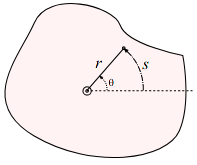
\includegraphics[width=0.5\textwidth]{7/fig/rot1.png}
    \caption{Um ponto no objeto que sofre rotação está localizado a uma distância $r$ do eixo; enquanto o objeto roda num ângulo $\theta$, o ponto move-se a distância $s$.}
\end{figure}

\subsubsection{Deslocamento Angular}
Conforme um objeto que roda se move através de um ângulo $\theta$ a partir da posição inicial, um ponto de massa no objeto no raio $r$ mover-se-á a distância $s$; $s$ é o comprimento do arco de um raio $r$ subtendido pelo ângulo $\theta$.

Quando $\theta$ está em radianos, as medidas acimas relacionam-se por

\begin{equation}
    \theta=\frac{s}{r} \qquad \theta \text{ em radianos}
\end{equation}

Se pensarmos na consistência das unidades na equação acima, verifica-se que dado que $s$ e $r$ ambos têm unidades de comprimento, $\theta$ não tem dimensão; but visto que estamos a assumir uma medida em radianos, normalmente escreve-se \emph{"rad"} depois do ângulo.

\subsubsection{Velocidade Angular}
A posição angular de um objeto muda com o tempo; tal como no movimento retilíneo, estudamos a variação de $\theta$ no tempo $t$. Se num período de tempo $\Delta t$ o objeto teve um deslocamento angular de $\Delta \theta$, então define-se a \textbf{velocidade angular média} para esse período como

\begin{equation}
    \bar{\omega}=\frac{\Delta \theta}{\Delta t}
\end{equation}

Uma quantidade mais interessante é encontrada quando se torna o período de tempo $\Delta t$ infinitesímal. Isto dá-nos a \textbf{velocidade angular instantânea}, $\omega$:

\begin{equation}
    \omega = \lim_{\Delta t \to 0}\frac{\Delta \theta}{\Delta t}=\frac{d\theta}{dt}
\end{equation}

A velocidade angular tem unidades $rad\ s^{-1}$ ou $s^{-1}$.

\subsubsection{Aceleração Angular; Aceleração Angular Constante}

A taxa à qual a velocidade angular muda é a aceleração angular do objeto. Se a velocidade angular instantânea de um objeto muda por $\Delta \omega$ durante um período de tempo $\Delta t$, então a \textbf{aceleração angular média} para este período é

\begin{equation}
    \bar{\alpha}=\frac{\Delta \omega}{\Delta t}
\end{equation}

A \textbf{aceleração angular instantânea} está definida como

\begin{equation}
    \alpha = \lim_{\Delta t \to 0}\frac{\Delta \alpha}{\Delta t}=\frac{d\omega}{dt}
\end{equation}

Podemos demonstrar equações simples para o movimento rotacional se soubermos que a $\alpha$ é constante. Então, se $\theta_0$ for o deslocamento angular inicial; $\omega_0$ for a velocidade angular inicial e $\alpha$ a aceleração angular constante, temos:

\begin{equation}
    \omega = \omega_0+\alpha t
\end{equation}

\begin{equation}
    \theta = \theta_0+w_0t+\frac{1}{2}\alpha t^2
\end{equation}

\begin{equation}
    \omega^2=w_0^2+2\alpha(\theta - \theta_0)
\end{equation}

\begin{equation}
    \theta = \theta_0 + \frac{1}{2}(w_0+w)t
\end{equation}

onde $\theta$ e $\omega$ são o deslocamento angular e a velocidade no instante $t$. $\theta_0$ e $\omega_0$ são os valores do ângulo e da velocidade angular em $t=0$.

As equações acima têm \emph{exatamente a mesma forma} que as equações para o movimento retilíneo em uma dimensão. As correspondências são:

$$
x \leftrightarrow \theta \qquad v \leftrightarrow \omega \qquad a \leftrightarrow \alpha
$$

\subsubsection{Relação Entre Qutnaidades Angulares e Lineares}
Quando um objeto que roda tem deslocamento angular $\Delta \theta$, então um ponto no objeto a um raio $r$ percorre uma distância $s=r\theta$. Isto é uma relação entre o movimento angular do ponto e o movimento "linear" do ponto. A distância do ponto desde o eixo não muda, por isso derivando esta relação em ordem ao tempo dá a velocidade instantânea da partícula:

\begin{equation}
    v=\frac{ds}{dt}=r\frac{d\theta}{dt}=r\omega
\end{equation}

que se chama a \textbf{velocidade tangencial}/\textbf{velocidade linear} $v_T$ do ponto para a distinguir da \emph{velocidade angular}. Note-se que todos os pontos do objeto que roda têm a mesma \emph{velocidade angular} mas as suas velocidades linear dependem da distância ao eixo de rotação.

Similarmente, a derivada em relação ao tempo da equação acima dá-nos a acelearção linear do ponto:

\begin{equation}
    a_T=\frac{dv}{dt}=r\frac{d\omega}{dt}=r\alpha
\end{equation}

Aqui, é essencial distinguir a aceleração \emph{tangencial} da aceleração \emph{centrípeta}. À semelhança do movimento circular uniforme, é verdade que um ponto a um raio $r$ terá a sua aceleração centrípeta dada por:

\begin{equation}
    a_c=\frac{v^2}{r}=\frac{(r\omega)^2}{r}=r\omega^2
\end{equation}

Estas duas componentes especificam o vetor aceleração de um ponto num objeto que sofre rotação.

\subsubsection{Energia Cinética de Rotação}
Porque a constituição de um objeto em rotação é feita de vários pontos de massa em movimento, este tem energia cinética; mas dado que cada ponto de massa tem uma velocidade $v$ diferente, a fórmula tradicional da energia cinética não se aplica. Se cada ponto de massa do objeto em rotação for denotado por $m_i$, cada um tendo velocidades lineares (diferentes!) $v_i$, então a energia cinética total do objeto em rotação é

\begin{equation}
    K_{r}=\sum_{i}\frac{1}{2}m_iv_i^2=\frac{1}{2}\sum_i m_iv_i^2
\end{equation}

Se $r_i$ for a distância do $i$-ésimo ponto de massa ao eixo, então $v_i=r_i\omega$ e temos:

\begin{equation}
    K_{r}=\sum_{i}\frac{1}{2}m_i(r_i\omega)^2=\frac{1}{2}()\sum_i m_i)\omega^2
\end{equation}

O somatório $\sum_i m_ir_i^2$ é chamada o \textbf{momento de inércia} para o objeto de rotação, e é usualmente denotado por $I$. Tem unidades do SI de $\kg\cdot m^2$. Com esta simplificação, a equação anterior torna-se

\begin{equation}
    K_{r}=\frac{1}{2}I\omega^2
\end{equation}

\subsubsection{Momento de Inércia; Teorema do Eixo Paralelo}
Para um objeto em rotação composto por vários pontos de massa, o \textbf{momento de inércia} $I$ é dado por

\begin{equation}
    I=\sum_i m_ir_i^2
\end{equation}

Tem unidades do SI de $\kg\cdot m^2$ e é um escalar (i.e. um único número que é sempre positivo). Mais frequentemente, lidamos com um objeto que é uma distribuição contínua de massa, e para este caso temos a expressão mais geral

\begin{equation}
    I=\int r^2dm
\end{equation}

Aqui, o integral é feito sob o volume do objeto e em cada ponto é computado $r^2$, onde $r$ é a distância medida perpendicularmente desde o eixo de rotação.

Supondo que o momento de inércia para um objeto de massa $M$ com o eixo de rotação a passar pelo centro de massa é $I_{CM}$. Agora, suponha-se que deslocamento o eixo paralelo a si próprio por uma distância $D$. O momento de inércia para o objeto sob o novo eixo de rotação terá um novo valor $I$, dado por

\begin{equation}
    I=I_{CM}+MD^2
\end{equation}

A equação acima é conhecida como o \textbf{Teorema dos Eixos Paralelos} e é, por vezes, útil para computar momentos de inércia se já tivermos um valor para o momento de inércia que passa pelo centro de massa do objeto.

\subsubsection{Torque}
É possível impactar a aceleração de um objeto em rotação exercendo uma força no mesmo num ponto em particular.

Supondo que a força \textbf{F} (cuja direção está no plano de rotação) é aplicado num ponto $r$ (relativo ao eixo de rotação que está na origem $O$). Supondo que o ângulo mais pequeno entre \textbf{r} e \textbf{F} é $\phi$. Então, a magnitude da \textbf{torque} exercida no objeto por esta força é

\begin{equation}
    |\tau|=rF\sin \phi
\end{equation}